\begin{recipe}
    [% 
        preparationtime = {\unit[15]{min}},
        bakingtime = {\unit[20]{min}},
        portion = {\portion{3-4}},
        source = {My Headmaster \& Giovanni Burro}
    ]
    {Pizza dough}

    \ingredients[8]{%
        \unit[150]{g} & wholemeal flour \\
        \unit[350]{g} & white flour \\
        \unit[25]{g} & fresh yeast \\
        \textbf{or} & \\
        \unit[7]{g} & dried yeast \\
        \unit[250]{ml} & milk \\
        \unit[2]{tbs.} & olive oil \\
        \unit[1]{ts.} & salt \\
        \unit[1]{ts.} & sugar
    }

    \preparation{%
        \step Warm up the milk to about \unit[40-50]{\textcelcius} and dissolve the yeast with sugar (hot water may kill the yeast!).
        Leave them to 'wake up' for \unit[5-10]{minutes}. You need a larger glass to accommodate some foam.

        \step Mix together the two types of flour, salt and oil.
        I prefer to start in a bowl, stirring with a table spoon.

        \step Gradually add the milk, stirring constantly.
        The dough should be sticky but not wet: balance with extra flour or warm water as needed.

        \step Put the dough on a flat, clean (Bethan, I'm watching you!)
        surface and pug for 5 minutes.
        The goal is to create bubbles of air inside so you should push the dough with the bottom of your palm(s) and them fold in half.
        \step Leave it to grow for at least 20 minutes in a warm place, covered with a cloth.
        Roll to \unit[3-5]{mm} thickness and bake for about 20 minutes at \unit[185]{\textcelcius} with your favourite toppings.
    
        \begin{figure}[h]
            \centering
            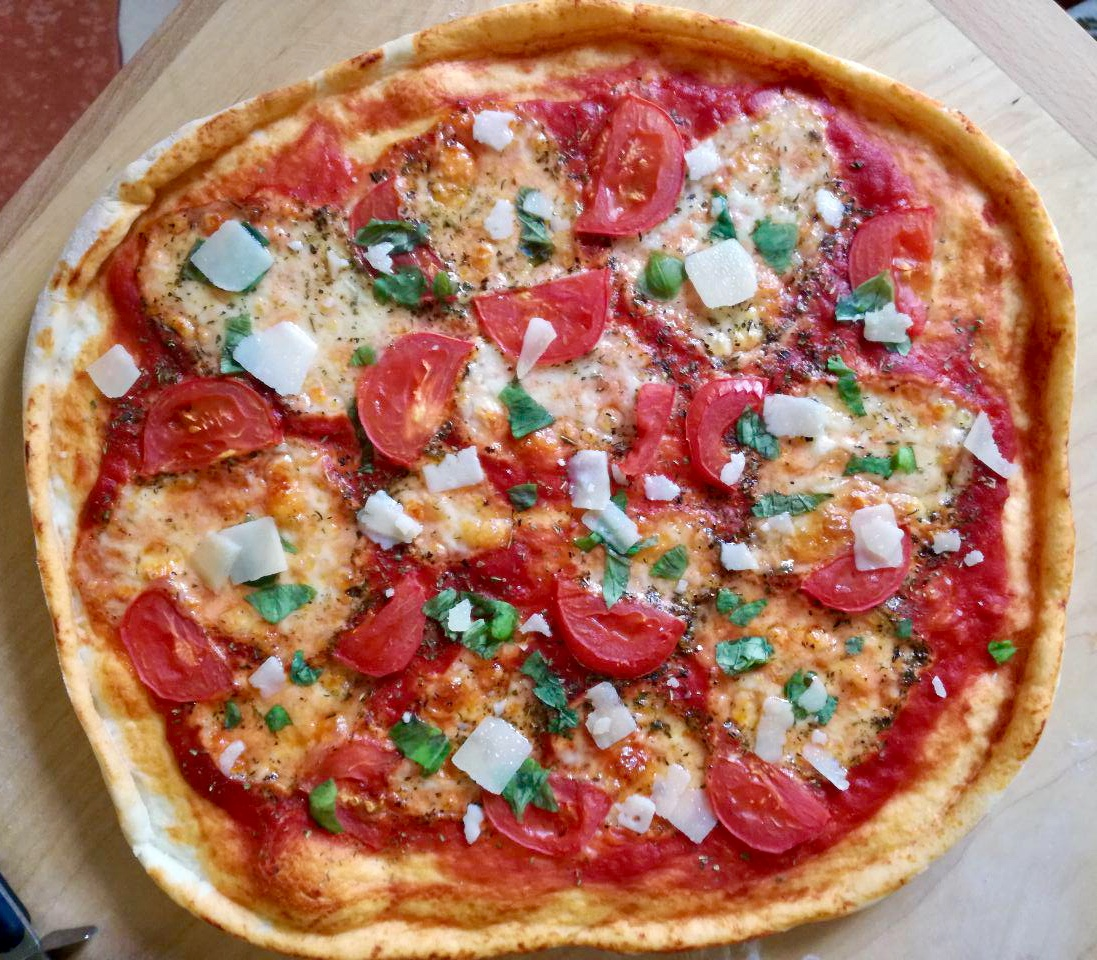
\includegraphics[width=12cm]{pic/pizza}
        \end{figure}
    }

    \hint{%
        Equation for yeast growth is exactly the same as for bacteria growth: moderate temperature, moisture, food, oxygen and time.
        That's why bacteria like washing-up sponges so much...
    }

\end{recipe}
